\graphicspath{{}{theory/}{Diagrams/}}


\section{The three neutrino paradigm}

Neutrinos provide the most compelling evidence for physics beyond the SM. In this chapter we explore why and discuss some of the most important properties of neutrinos for their experimental study.

Neutrinos are purely weakly interacting fields

Neutrinos -- Pauli + Madame Wu + Freinberg numus + Lederman

\section{Oscillations}

Neutrino oscillations can arise when a superposition of neutrino mass eigenstates is produced, propagates macroscopic distances and scatters inside a detector. Given sufficiently long baselines, neutrino flavour transitions may always occurs due to mixing, but for a sinusoidal dependence on baseline coherence must be preserved throughout the process. We will now derive the standard formula for the oscillation probability in vacuum, $P(\nu_\alpha \to \nu_\beta)$ (matter effects are discussed in \refsec{sec:matter_effects}). This exercise can be done in multiple ways and most often derivations will rely on the neutrino states to be plane-wave solutions. This approach leads to correct expressions for $P(\nu_\alpha \to \nu_\beta)$ in virtually all cases of interest, but it is a rather poor conceptual description of oscillations and a very limited framework. Instead we will derive the oscillation formula starting from a quantum mechanical wave-packet approach, and encounter a few conditions for oscillations to happen. More sophisticated treatments in Quantum Field Theory (QFT) have been known for some time~\cite{Cardall:1999ze,Beuthe:2001rc,Giunti:2002xg}, and their results have been shown to be directly mapped onto the wave-packet approach~\cite{Akhmedov:2010ms}. Nonetheless, neutrino oscillations are notorious for being conceptually confusing and the correct method to compute such processes is still debated in the literature~\cite{Kobach:2017osm}. One may seek consolation in the fact that a few aspects are common to all approaches, for instance the ultra-relativistic nature of the mass states through expansions of $\sqrt{m^2 + p^2}$ and the need for momentum uncertainties in the initial and final neutrino processes.

%
\begin{figure}[t]
\centering
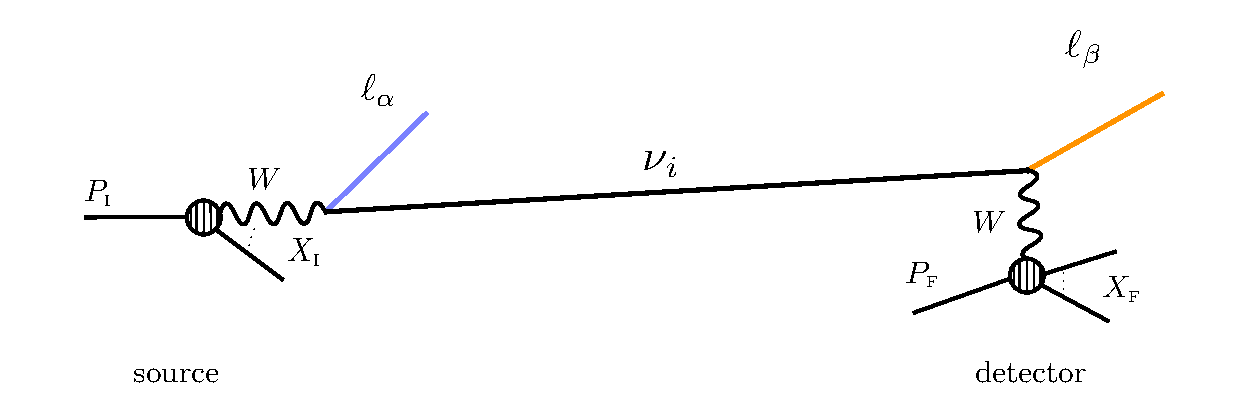
\includegraphics[width=\textwidth]{oscillations_diagram.pdf}
  \caption[Neutrino oscillations diagram.]{The usual set-up of an oscillation experiment. We show the source, where a process $P_\textsc{i} \to \nu_\alpha \, X_\textsc{i}$ happens (note that $P_\textsc{i}= \ell_\alpha$ is allowed and that $P_\textsc{i}$ may be a scattering process), and the detector, where $\nu_\beta \,P_i \to \ell_\beta \,X_\text{f}$. \label{fig:oscillations_diagram}}
\end{figure}
%
Our setup is the same as most neutrino oscillations experiments and is represented in \reffig{fig:oscillations_diagram}. We will first discuss the production and detection processes, and then study the oscillations per se. Initially, a neutrino flavour state $\nu_\beta$ is produced by a CC reaction at the source, $P_\textsc{i} \to \nu_\beta X_\textsc{i}$. More precisely, a state $\bra{f}$ is produced,
%
\begin{equation}\label{eq:flavour_source}
 \ket{f} = \hat{S} \ket{P_\textsc{i}}, \quad \hat{S} \approx  \hat{1} - i \int \dd^4 x \, H_{\rm int}^{\rm CC} (x),
\end{equation}
%
where $\hat{S}$ is the S-matrix operator approximated to first order in weak coupling and
%
\begin{equation}
 H_{\rm int}^{\rm CC} (x) = \sqrt{2} G_F\, \sum_\alpha \overline{\nu}_\alpha (x) \gamma^\mu P_L \ell_\alpha(x) \, J_\mu (x) \,+\, {\rm h.c.},
\end{equation}
%
is the interaction Hamiltanian between the neutrino current and the current $J_\mu(x)$ that describes the transition $P_\textsc{i} \to X_\textsc{i}$. After $\ell_\alpha$ and the final particles interact with the medium, $\bra{f}$ is reduced to $\bra{\ell_\alpha,\,X_\textsc{i}}\ket{f}$, which ought to ensure that only neutrino flavour states $\nu_\alpha$ are produced, according to our flavour basis definition. Unfortunately, flavour states are not well-defined and do not span a Fock space. We want to work instead with the eigenstates of the free Hamiltonian, which are the ones we can easilly evolve in time. With this in mind, we define the following amplitude
%
\begin{equation}
 A_{\alpha k}(\vec{p},h)^P \equiv \bra{\nu_k(\vec{p},h),\ell_\beta,X_{\textsc{i}}} \hat{S}\ket{P_\textsc{i}}, \quad {\rm with} \quad A_{\alpha k}(\vec{p},h) = U^*_{\alpha k} M_{\alpha k}(\vec{p},h),
\end{equation}
%
where we factored out a mixing angle in the definition of $M_{\alpha k}$ and made the helicity index $h$ explicit. By virtue of the completeness relation with massive neutrino eigenstates, we can insert the identity in $\bra{\ell_\alpha,\,X_\textsc{i}}\ket{f}$ and define a \emph{normalized} neutrino flavour state as
%
\begin{equation}
 \ket{\nu_\alpha}^P = N_P \,\sum_{k, h} \, \int \dd^3 p\, A^P_{\alpha k} (\vec{p},h) \ket{\nu_k(\vec{p},h)}, \quad N_P^{-2} = \sum_{k,h} \int \dd^3 p \, \left|A^P_{\alpha k} (\vec{p},h)\right|^2.
\end{equation}
%
An analogous discussion holds for the detection process $\nu_\beta \, P_\textsc{f} \to \ell_\beta \, X_\textsc{f}$, where a detection flavour state $\ket{\nu_\alpha}^D$ with an amplitude for detection $A_{\alpha k}(\vec{p},h)^D$ can be defined. Before we move on to a discussion about oscillations, we want to emphasize two points. First, the normalization of the flavour state is a clear sign that we are working in a quantum mechanical description. To compute probabilities, we rely on normalized states. In a QFT description, however, the normalization is not necessary, but so is the concept of $P_\textsc{i} \to X_\textsc{i}$ in the first place. There, the full process in \reffig{fig:oscillations_diagram} can be compute directly through the use of long-distance propagators, and if the production, propagation and detection parts of the amplitude squared factorize, an object equivalent to the oscillation probability can be extracted. This factorization is implicitly assumed in our calculation. Secondly, the decay rate of the $P_\text{I}$ particle can be computed as
%
\begin{equation}
 \left|A^P\right|^2 =  \left|  \bra{\nu_\alpha (\vec{p},h),\ell_\beta, X_{\textsc{i}}} \hat{S} \ket{P_\textsc{i}}  \right|^2 = \sum_{k,h} \,|U_{\alpha k}|^2\, \int \dd^3 p \, \left|M^P_{\alpha k} (\vec{p},h) \right|^2,
\end{equation}
%
and it becomes evident that the decay rate is given by the \emph{incoherent} sum of the decay rate into different massive neutrinos. No interference is present as the states $\ket{\nu_k}$ are assumed to be orthonormal to each other. This remains true in the QFT description~\cite{Giunti:2002xg}.

Now, one is left to compute the functions $M_{\alpha k}$. This is a rather involved process, but one can show that the form of these functions resemble simple wavepackets~\cite{Akhmedov:2010ms}. In doing so, many approximations are necessary, in particular, that of ultra-relativistic neutrinos. More precisely, the most relevant assumptions are \emph{i)} flipped-helicity terms ($h=+$ for neutrinos), suppressed by $m_k^2/E_k^2$, are ignored, \emph{ii)} all neutrinos travel in the same direction, $\vec{p} \to p$, and \emph{iii)} the production and detection processes are not sensitive to the neutrino mass differences, amounting to replacing $M_{\alpha k} \approx M_\alpha$. Under these assumptions, we are justified to take normalized gaussian wavepackets for production and detection flavour states as an \emph{ansatz},
%
\begin{equation}
 \ket{\nu_\alpha}^i =  \sum_{k}  U^*_{\alpha k} \, \int \dd p \, \psi_k^i (p) \,\ket{\nu_k({p})}, \quad%
 %
 \psi_k^i (p) = \left(2\pi\,\sigma_p^{i\, 2}\right)^{-1/4} \exp\left[ - \frac{(p-p_k)^2}{4 \sigma_p^{i\, 2}} \right],
\end{equation}
%
with $\sigma_p^i$ being the spread around the central momenta $p_k$ and $i=P,D$.

Now that the flavour states are written in terms of the eigenstates of the free Hamiltonian, we know how to evolve them and how to write the flavour transition amplitude after a time $t$ and distance $L$
%
\begin{align}
 A(\nu_\alpha \to \nu_\beta) &= \bra{\nu_\beta^D} e^{-i \hat{E} t + i \hat{P} L} \ket{\nu_\alpha^P}
 \nonumber \\ &= N \,\sum_k U_{\alpha k}^* U_{\beta k} \int \dd p \exp\left[ -i E_k(p) t + ip L - (p -p_k)^2/4 \sigma_p^2\right],
\end{align}
where $E_k(p) = \sqrt{p^2 + m_k^2}$ and N is a normalization factor coming from the normalization of the wavepackets and a single integral over $p$. We have also defined the global energy uncertainty on momentum $\sigma_p^{-2} = \left(\sigma_p^{P}\right)^{-2} + \left(\sigma_p^{D}\right)^{-2}$. This may also be related to the global uncertainty on production and detection positions through $\sigma_x \sigma_p \approx 1/2$. Finally, to integrate over the remaining $p$ integral, we can taylor expand around the central wavepacket momentum
%
\begin{equation}
 E_k(p) \approx E_k + v_k (p-p_k), \quad{\rm with}\quad v_k = \left.\frac{\partial E_k(p)}{\partial p}\right|_{p=p_k} = \frac{p_k}{E_k},  \quad E_k = \sqrt{p_k^2 + m_k^2}.
\end{equation}
%
Perfomrming the final integral over $p$, integrating over $t$ (an unmeasured quantity) and squaring the amplitude, one obtains a formula for the oscillation probability
%
\begin{equation}
 P(\nu_\alpha \to \nu_\beta) = \sum_{k,j} U_{\alpha k}^*U_{\alpha j}U_{\beta k}U_{\beta j}^* \, e^{-2\pi i L/L^{\rm osc}_{kj}} \, P^{\rm coh}_{kj} \, P^{\rm loc}_{kj},
\end{equation}
%
where we defined
%
\begin{equation}
  P^{\rm loc}_{kj} = \exp\left( -2 \pi^2 \xi^2 \left(\frac{\sigma_x}{L_{kj}^{\rm osc}} \right)^2 \right),\quad  P^{\rm coh}_{kj} = \exp\left( \frac{L \left|\Delta m^2_{kj} \right|^2}{16 E^2 \sigma_x} \right),
\end{equation}
%
and the important scales of the problem can be identified as
%
\begin{equation}
 L_{kj}^{\rm osc} = \frac{4 \pi E}{\Delta m_{kj}^2}, \quad  p_k \approx E - (1-\xi) \frac{m_k^2}{2E}, \quad E_k \approx E + \xi \frac{m_k^2}{2E},
\end{equation}
with $\xi$ measuring the deviation from ultra-relativistic behaviour.
%

For most application, $P^{\rm coh}_{kj} = P^{\rm loc}_{kj} = 1$, and one recovers the standard oscillation formulae. A more useful way of writing it is
%
\begin{align}
 P(\nu_\alpha \to \nu_\beta) =
 \delta_{\alpha\beta} &- 2\sum_{k>j} \Re{U_{\alpha k}^*U_{\alpha j}U_{\beta k}U_{\beta j}^*} \left[ 1- \cos\left( \frac{\Delta m^2_{kj} L}{2E}\right) \right] \nonumber\\
 %
 &- 2\sum_{k>j} \Im{U_{\alpha k}^*U_{\alpha j}U_{\beta k}U_{\beta j}^*} \sin \left( \frac{\Delta m^2_{kj} L}{2E}\right) 
\end{align}
%

\subsection{Matter effects}\label{sec:matter_effects}

Neutrinos are neutral particles and their rare interactions allow them to propagate through matter without losing energy in collisions with the medium particles. Nevertheless, in a similar fashion to photons, neutrinos undergo coherent forward scattering, acquiring an effective refractive index in the presence of a medium. In contrast to photons, which undergo Compton scattering, neutrinos are only charged under the weak force and can only undergo CC or NC interactions. The weakness of these interactions at low energies implies that matter effects arise only when neutrinos have transversed sufficiently large distances or are in a sufficiently dense environment. In principle, for large matter effects all that is necessary is a net weak charge for the medium, provided by the neutrons in the case of the Earth. However, for such effects to be observable in neutrino oscillation experiments, an additional condition exists: different flavour states must exhibit different interaction potential with the medium. In the SM, this is possible due to the CC interactions that are exclusively between electron-neutrino states and electrons in the medium.

The time evolution of the flavour states is again given by the Schr\"oedinger equation in the presence of an interaction potential
%
\begin{equation}\label{eq:matter_evolution}
 i \frac{\dd}{\dd x} \ket{\nu_\alpha} = \left[ U \frac{\hat{m}^2}{2E} U^\dagger + \hat{V}(x) \right] \ket{\nu_\alpha}, 
\end{equation}
%
where we have already used the ultra-relativistic approximations from before, applying $H_0 \ket{\nu_\alpha} \approx U \left[ p \hat{1} + \hat{m}^2/2 p \right] U^\dagger \ket{\nu_\alpha} $ and $t \approx x$. Solving this equation is a much more complicated task than in the vacuum case. Full analytical solutions are only known in specific cases, such as when the column density of matter particles is constant~\cite{}. In general, this may be solved numerically for a given choice of $\hat{V}$, although several perturbative expansions exist~\cite{}. 

Various calculations of the neutrino matter potential exist, but often these rely on averages over the particle background and are difficult to generalize to non-standard cases. Here, we sketch the approach of Refs.~\cite{Notzold:1987ik,Nieves:1989ez}, where the neutrino potential arises from finite temperature and finite density corrections to the neutrino dispersion relation. In particular, the dispersion relations arises from
%
\begin{equation}
 \det{\slashed{k} - \Sigma} = 0,
\end{equation}
%
guaranteeing non-trivial solutions to the Dirac equation $(\slashed{k} - \Sigma)\nu_L = 0$, with $k^\mu$ the neutrino four-momentum and $\Sigma$ its self-energy. For LH neutrino states $\nu_L$, we can write the neutrino self-energy in the most general form and make explicit the background dependent contribution as~\cite{Weldon:1982aq}
%
\begin{equation}
  \Sigma = m - \left( a_L \slashed{k} + b_L \slashed{u} + c_L [\slashed{k},\slashed{u}] \right) P_L.
\end{equation}
%
where $u$ is the 4-velocity of the medium, $a_L,b_L$ and $c_L$ are scalar functions of Lorentz invariants $w=k \cdot u$ and $\kappa=(w^2 - k^2)^{1/2}$, and $m$ is the vacuum neutrino mass. The presence of the medium introduces a preferential frame, namely the rest frame of the medium with $u = (1,0,0,0)$. Also note that in vacuum, only terms proportional to $\slashed{k}$ exist, and the pole of the neutrino propagator is unchanged. To lowest order, $g^2/m_\textsc{w}^2$, only $b_L$ contributes and it is proportional to the medium particle-antiparticle asymmetry, both statements not holding for higher order terms of the form $g^2/m_\textsc{w}^4$~\cite{DOlivo:1992lwg}. The neutrino self-energy is in fact a gauge-dependent quantity, so the physical observables of interest are the dispersion relations, $(1-a_L)(w-\kappa)- b_L = 0$ for neutrinos and $(1-a_L)(w+\kappa) - b_L = 0$ for antineutrinos. To lowest order, however, the dispersion relations are much simpler,
%
\begin{equation}
 w \approx \kappa + \frac{m^2}{2\kappa} + V_{\rm eff}, \quad V_{\rm eff} = -b_L,
\end{equation}
%
where we defined the effective potential, which for ultra-relativistic neutrinos arises precisely from the difference between the total and kinetic energy $V_{\rm eff} = w - \kappa$. This also shows us how to calculate the neutrino refractive index $n =|\vec{k}|/k^0$.
%
\begin{figure}[t]
 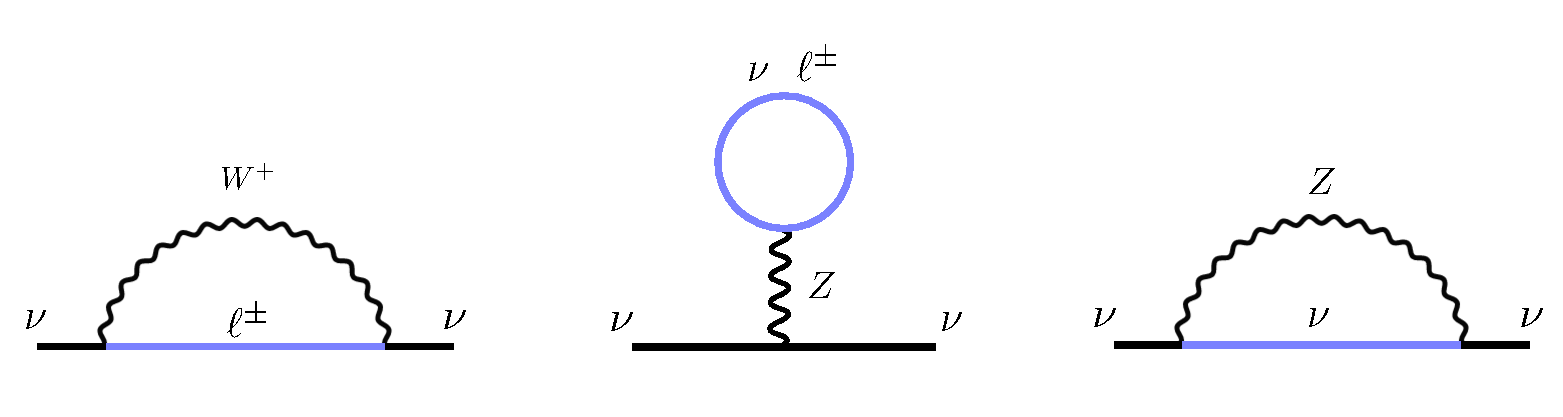
\includegraphics[width=\textwidth]{thermal_diagrams.pdf}
  \caption[Finite temperature corrections to $\Sigma$.]{Finite temperature and density corrections to the neutrino self-energy. These can be used to infer the effective matter potential for neutrinos.\label{fig:thermal_diagrams}}
\end{figure}

Now the problem reduces to computing $\Sigma$ in finite temperature field theory. For most applications of thermal mass calculations, replacing vacuum propagators by the thermal propagators from the real-time formalism is sufficient. In particular, the fermion thermal propagator of interest is
%
\begin{equation}
 S(P) = (\slashed{p} + m)\left[ \frac{1}{P^2 - m^2 +i\epsilon } + i 2\pi \delta(P^2 - m^2) f(P)\right],
\end{equation}
%
with $f(P) = \left\{ \exp\left[(|P\cdot u| - {\rm sgn}(P \cdot u) \,\mu_f)/T\right] + 1\right\}^{-1}$ is the occupational number of the fermions in the thermal bath of temperature $T$ and chemical potential $\mu_f$. Similar expressions exist for bosonic propagators. Finally, as an example, explicit computation of the self-energy in \reffig{fig:thermal_diagrams} yields
%
\begin{equation}
 \Sigma = -i \frac{g^2}{16 c_\textsc{w}^2}\int \frac{\dd^4 P}{(2\pi)^4} \gamma^\mu P_L \,iS(P+K) \,\gamma^\nu \, P_L \,iD_{\mu\nu} (P),  \quad D_{\mu\nu} = \frac{-g_{\mu\nu} + \frac{P_\mu P_\nu}{M_Z^2}}{P^2 - M_Z^2 + i\epsilon}.
\end{equation}
%

Putting it all together, the potential for neutrinos of flavour $\alpha$ on a background of protons, neutrons and electrons is
%
\begin{align}
 V^e_\alpha =& -\frac{G_F}{\sqrt{2}} \left( 2\delta_{\alpha e} 1-4s^2_\textsc{w} \right) \left( N_e - N_{\overline{e}} \right),\nonumber\\%
 V^p_\alpha =& \frac{G_F}{\sqrt{2}} \left( 1-4s^2_\textsc{w} \right) \left( N_p - N_{\overline{p}} \right),\nonumber\\%
 V^n_\alpha =& -\frac{G_F}{\sqrt{2}} \left(N_n - N_{\overline{n}} \right).
\end{align}
%
For antineutrino an overall minus sign is introduced. Note the $\nu_e$ potential is the only one where CC interactions contribute, and so it is the sole responsible for non-trivial flavour evolution in \refeq{eq:matter_evolution}. One may wonder about radiative corrections to these potentials in the SM and whether additional flavour non-universality can be achieved through the difference in charged-lepton masses. These effects, however, are known to be extremely small in the SM~\cite{Botella:1986wy}, where $\left(V_\tau - V_\mu\right)/V_e \approx 5 \times 10^{-5}$ for a neutral unpolarized medium like the Earth. 


\section{The model space of neutrino physics}

A more ambitious task than measuring the low-energy properties of neutrinos is to understand the theoretical origins of neutrino mass and mixing. Here, the possibilities are manifold. The high-scale dynamics, typical of many neutrino mass models, is incredibly hard to test, so it is fair to say we have more neutrino mass models than ways to test them. Nevertheless, many of these models possess similar features. They may rely on the seesaw mechanism, on radiative neutrino mass generation or in extended scalar sectors. On top of that, new symmetries and fundamental forces may also be at play. We will explore a small fraction of this model space.

\subsection{Mass mechanisms}

\begin{figure}[t]
\centering
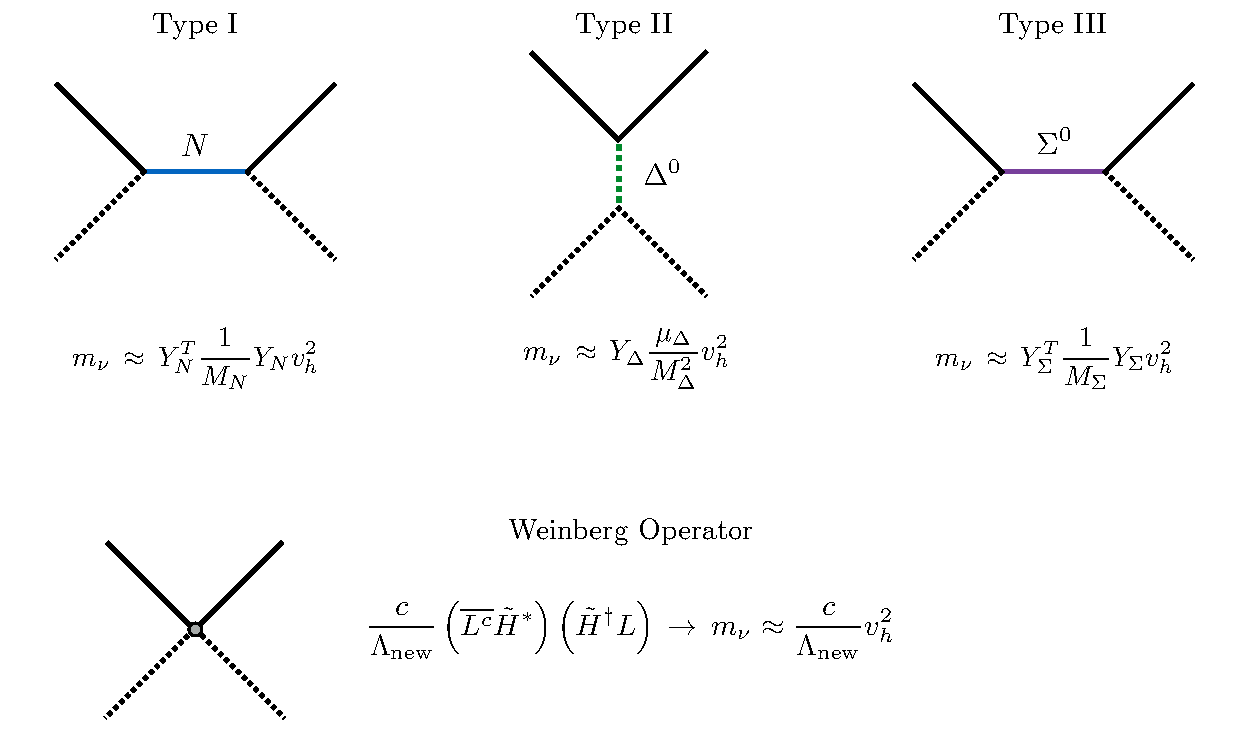
\includegraphics[width=\textwidth]{seesaw_mechanisms.pdf}
\caption[The tree-level UV completions of the Weinberg operator.]{The only three UV completions of the $d=5$ Weinberg operator with their respective contributions to light neutrino masses.\label{fig:seesaw_mechanisms}}
\end{figure}


In \reffig{fig:seesaw_mechanisms}, we show these unique tree-level completions of the Weinberg operator.

For a review on low-scale models see \cite{Boucenna:2014zba}.

\subsection{Conventional seesaws}

\subsection{Low scale seesaw variants}

\subsection{Radiative masses}

The most straightforward extension of the SM which can generate neutrino masses at loop level is perhaps the so-called Zee-Babu model.

\subsection{Sources}\label{sec:sources}

To find a source of neutrinos, all we have to do is to look for environments where the Weak force is prominently manifested. A natural candidate, as we have seen in the discovery of the neutrino, are nuclear reactors. Fortunately, the list does not stop there. Abundant neutrino sources include the Sun, the atmosphere, the Big-Bang, particle accelerators and astrophysical environments processes such as supernovae, active galactic nuclei and others. 

\section{Scattering}

Neutrino cross sections are an invaluable observable to understand the weak force and to search be able to study oscillation physics. Due to the purely weakly interacting nature of neutrinos, they also serve as a strong test of \emph{stronger than weak} interactions with matter, that is, new interactions with $G_X > G_F$. In fact, if sufficiently clean, neutrino scattering processes provide the strongest limits on light new mediators of masses from a few MeV to a few GeV~\cite{}. In this section, we present the standard scattering channels used in oscillation experiments, as well as other curious processes that are relatively poorly studied. 

Accelerator experiments typically produce neutrinos of a few GeV energies to achieve $\mathcal{O}(1)$ oscillation phases $\Delta m^2_{\rm atm} L/E$ within thousands of km. Drastically different energy regimes are impractical either due to diluted fluxes at longer baselines ($\Phi \propto 1/L^2$), or due to thresholds to produce muons in CC interactions ($E_\nu > m_\ell + m_\ell^2/2 m_{\mathcal{H}}$ in reactions of the type $\nu_\ell \mathcal{H} \,\to\, \ell^\pm \mathcal{H}^\prime$). Also important is the fact that such experiments rely on the neutrino flux produced in proton-on-target collisions, where charged mesons are subject to magnetic fields for focusing (see \refsec{sec:sources}). This produces neutrinos with a wide spectrum, typically referred to as wide-band-beam spectram, and are hard to model due to hadroproduction and focusing uncertainties~\cite{}. In this way, the expected neutrino event rate in neutrino detectors inherits two sources of uncertainties which are difficult to disentangle: the un-oscillated flux spectra and the neutrino-nucleus cross sections. The latter observable is subject to large nuclear effects, which require either precision data or accurate descriptions of the nuclear environment. 

Take the MiniBooNE experiment, for instance, where the average neutrino energy is $\langle E_\nu \rangle \approx 800 $ MeV. The nucleons struck by the neutrinos in the processes of interst are inside Carbon nuclei, and so their interactions with the nuclear medium are important. Even in the crudest approximation for a nucleus, that of a $T=0$ Fermi gas of free protons and neutrons, nucleons may have quite large momenta in the rest frame of the nucleus, $|p| \lesssim 250 MeV$, being comparable to the incoming neutrino energies. In addition to fermi motion, the Pauli exclusion principle suppresses possible final state configurations in the nucleus. Pauli blocking.  possibly exchanging EM charges, knocking-out additional particles or being absorbed in the nuclear medium. The importance of nuclear effects is perhaps most famously illustrated by the CCQE measurement at MiniBooNE~\cite{AguilarArevalo:2010zc}, where a disagreement of $20\%$ was observed between the MC prediction and the data, unless the axial mass $M_A$ was set to be $\approx1.32$ GeV, much larger than the world-average of $M_A = 1.03 \pm 0.02$ GeV. This was later understood as a missing contribution from two-particle two-hole meson exchange currents (where the neutrino interacts with a nucleon pair, rather than with an individual nucleon), shown to be as large as $30\%$ of the CCQE cross section used by the experiment~\cite{Nieves:2011yp}.

Currently several neutrino event generators exists, the most popular being GENIE~\cite{Andreopoulos:2009rq}, GiBUU~\cite{Buss:2011mx}, NEUT~\cite{Hayato:2002sd} and NuWro~\cite{Juszczak:2005zs}.
